% !TEX program = lualatex
% !TEX encoding = utf-8
% !BIB program = biber
% !TEX spellcheck = it_IT

% !TEX program = lualatex
% !TEX root = ./tlinstall.tex

\documentclass[ structure = article
              , secnumstyle = dotarabic
              , liststyle = aligned
              , headerstyle = authortitlecenter
              ]{suftesi}

% gestione font
\usepackage[no-math]{fontspec}
\setmainfont{Linux Libertine O}
\setsansfont{Ubuntu}[Scale=MatchLowercase]
\setmonofont{Ubuntu Mono}[Scale=MatchUppercase]
\usepackage{anyfontsize}

% gestione lingue
\usepackage{polyglossia}
\setmainlanguage{italian}

% virgolette
\usepackage[autostyle,italian=quotes]{csquotes}
\newcommand\q\enquote

% riferimenti incrociati
\usepackage{hyperref}
\hypersetup{ breaklinks
           , hidelinks
           , linktocpage
           }

% bibliografia
\usepackage[backend=biber]{biblatex}
\addbibresource{mybib.bib}
\nocite{*}

% immagini
\usepackage{graphicx}
\graphicspath{{figure}}

% codici
\usepackage{listings}
\lstset{ basicstyle      = \ttfamily
       , escapeinside    = {?!}{!?}
       , escapebegin     = {\normalfont\em$\langle$\kern-1pt}
       , escapeend       = {$\rangle$}
       , backgroundcolor = \color{gray!10!white}
       }

% abstract
\usepackage{abstract}

% comandi personali
\newcommand\texlive{\TeX{}{\em live}}
\newcommand\gnulinux{{\sf GNU/Linux}}

% tasti tastiera
\usepackage{menukeys}
\newcommand\invio{\keys\return}


\title{Installare \texlive{} su \gnulinux{}}
\author{Indrjo Dedej}
\date{Ultima revisione: \today}

\begin{document}
\maketitle
% !TEX program = lualatex
% !TEX spellcheck = it_IT
% !TEX root = ../tlinstall.tex

\section{Installazione}

\begin{enumerate}

\item Bisogna scaricare il file \lstinline£texlive.iso£. Andare su
\begin{center}
\url{http://www.tug.org/texlive/acquire-iso.html}
\end{center}
e poi cliccare su {\sf Download from a nearby CTAN mirror}.\footnote{Su questo primo passo si può dire una cosa: di fatto, è una porta in faccia a chi avvicina per la prima volta al mondo di \TeX{}. Questo perché ci sono casi in cui i tempi di scaricamento della \lstinline£.iso£ possono essere terribilmente, impossibilmente ed insopportabilmente lunghi, a seconda dei capricci della rete e dalla lentezza dei {\em mirrors} che distribuiscono \texlive{}. Quindi: pazienza... D'altra parte sono 3GB e rotti di peso... È forse questo l'ostacolo maggiore dell'installazione.}

\item Creiamo la cartella \lstinline£iso£ all'interno della cartella \lstinline£media£
\begin{lstlisting}
sudo mkdir /media/iso
\end{lstlisting}
e montiamoci \lstinline£texlive.iso£
\begin{lstlisting}
sudo mount -o loop ?!dove si trova!?/texlive.iso /media/iso
\end{lstlisting}
Di solito quello che si scarica col browser va a finire in \lstinline£~/Scaricati£.

\item Possiamo iniziare l'installazione
\begin{lstlisting}
sudo /media/iso/install-tl
\end{lstlisting}
Durante questo processo non sono richiesti particolari interventi dall'utente: quando viene chiesto dal terminale quale tipo di installazione effettuare, scegliere quella completa digitando {\sf I} (la lettera \q{i} maiuscola) e premendo il tasto \invio{}.\footnote{Questo passaggio per essere portato al termine con successo richiede un po' meno tempo: dai 15 ai 20 minuti.} Potrebbe essere utile sapere che tutto quello che viene installato di default va a finire in \lstinline£/usr/local/texlive£.

\item Finita l'installazione \lstinline£texlive.iso£ non ci serve più, perciò smontiamolo
\begin{lstlisting}
sudo umount /media/iso
\end{lstlisting}
e possiamo eliminare anche la cartella \lstinline£/media/iso£
\begin{lstlisting}
sudo rm -rf /media/iso
\end{lstlisting}

\item Impartiamo il seguente comando
\begin{lstlisting}
xdg-open ~/.bash_aliases
\end{lstlisting}
che apre una pagina di file di testo.\footnote{Questo file può darsi che non esista (anzi è probabile che non esista) e quindi bisogna crearselo: si può fare col comando \lstinline£touch ~/.bash_aliases£.} Copiamo alla fine del file che viene aperto le seguenti righe:
\begin{lstlisting}
texlive="/usr/local/texlive/?!anno!?"
PATH=$texlive/bin/x86_64-linux:$PATH
export PATH
MANPATH=$texlive/texmf-dist/doc/man:$MANPATH
export MANPATH
INFOPATH=$texlive/texmf-dist/doc/info:$INFOPATH
export INFOPATH
\end{lstlisting}
Salviamo ed chiudiamo la finestra. Facciamo assimilare le novità introdotte:
\begin{lstlisting}
. ~/.bash_aliases
\end{lstlisting}

\item Fine :)
\end{enumerate}

% !TEX program = lualatex
% !TEX spellcheck = it_IT
% !TEX root = ../tlinstall.tex

\section{Manutenzione}

\begin{figure}
\centering
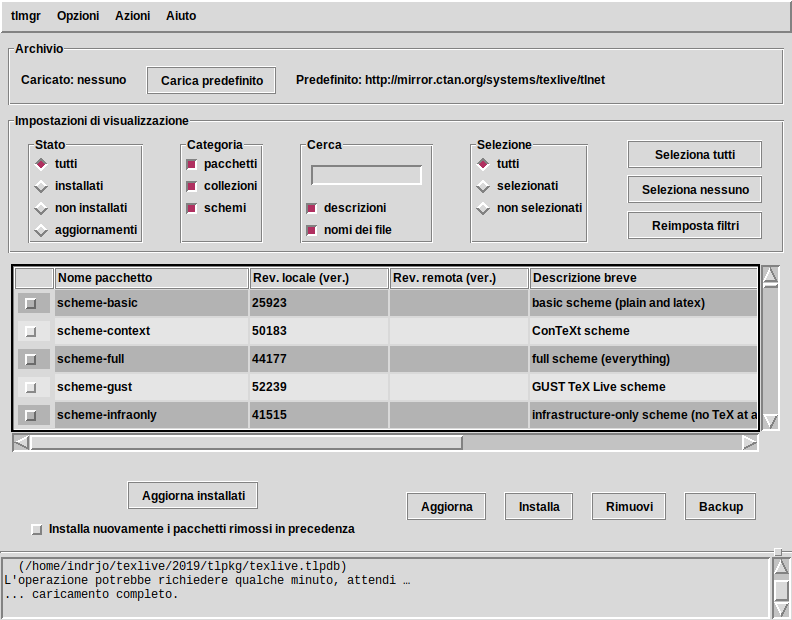
\includegraphics[width=.7\textwidth]{tlmgr}
\caption{\tt tlmgr gui}
\label{fig:gui}
\end{figure}

Diamo qualche breve suggerimento per la manutenzione di \texlive{}. Il programma che ci aiuta in ciò si chiama {\sf tlmgr}. Per averlo pronto all'uso, in fondo al file \lstinline£~/.bash_aliases£ aggiungiamo
\begin{lstlisting}
alias tlmgr='sudo env PATH=$PATH tlmgr'
\end{lstlisting}
da usare nel terminale come
\begin{lstlisting}
tlmgr ?!qualcosa!?
\end{lstlisting}
L'azione che vogliamo insegnare in questa sede è quella dell'aggiornamento dei pacchetti. Per aggiornare se stesso (perché qualche volta ne ha bisogno) dare
\begin{lstlisting}
tlmgr update --self
\end{lstlisting}
Per sapere quali pacchetti hanno bisogno di essere aggiornati (nessuno ci obbliga ad aggiornarli, ma è sempre meglio farlo) fare eseguire questo comando
\begin{lstlisting}
tlmgr update --list
\end{lstlisting}
e per aggiornare tutti quelli che sono aggiornabili
\begin{lstlisting}
tlmgr update --all
\end{lstlisting}
Il consiglio è, finita la procedura di installazione, di aggiornare {\sf tlmgr} stesso e di aggiornare, se possibile, tutti i pacchetti aggiornabili: questo perché nella \lstinline£texlive.iso£ tutto è congelato allo stesso e identico stato del rilascio, col rischio di trovarsi materiale non aggiornato. Se si vuole aggiornare un singolo pacchetto, si può usare
\begin{lstlisting}
tlmgr update ?!nome pacchetto!?
\end{lstlisting}

%\begin{nota}
Se il terminale fa ancora paura, si può optare per questa alternativa
\begin{lstlisting}
tlmgr gui
\end{lstlisting}
che apre la finestra in figura~\ref{fig:gui}. Da lì si possono fare tutte le azioni appena viste e anche altre. Serve che ci sia il modulo {\sf Tk}, però: per installarlo da terminale
\begin{lstlisting}
cpan -f Tk
\end{lstlisting}
%\end{nota}

% !TEX program = lualatex
% !TEX spellcheck = it_IT
% !TEX root = ../tlinstall.tex

\section{Disinstallazione}

Può succedere che, per un motivo o un altro, si voglia disinstallare \texlive{}. In realtà, sicuramente dovrete fare questa manovra: infatti, per passare da una versione alla successiva, bisogna eliminare la distribuzione installata per fare posto alla nuova.\footnote{I rilasci avvengono annualmente in primavera. Solitamente gli utenti tendono a tenersi la versione vecchia per qualche mese per poi fare queste operazioni durante l'estate. In tutto questo potrebbe esserci una qualche consolazione: siete in periodo di pausa e quindi questo avanzamento di versione non vi toglierà (si spera) troppo tempo al vostro lavoro. Uno potrebbe pensare di non avanzare di versione, ma questa scelta si paga visto che le vecchie versioni non ricevono più aggiornamenti. Si consiglia di assecondare questo ciclo di \q{creazione e distruzione}, quanto meno avere pazienza e sperare in dei cambiamenti.} Ci sono principalmente due vie: 
\begin{enumerate}
\item per via grafica: sulla barra superiore della finestra in figura~\ref{fig:gui}, premere {\sf Azioni}, che aprirà un menù a tendina, e poi {\sf Rimuovi TeXlive}.
\item manualmente, come suggerito in~\cite{exch:uninstall}.
\end{enumerate}
Io consiglio il secondo metodo: sebbene molto lungo e scomodo, fa una pulizia meticolosa di \texlive{}.
\printbibliography
%% !TEX program = lualatex
% !TEX spellcheck = it_IT
% !TEX root = ../tlinstall.tex

~\vfill
\begin{center}
\begin{tabular}{p{.8\textwidth}}
Tutto il lavoro è depositato su {\sf Github} all'indirizzo
\begin{center}
\url{https://github.com/indrjo/TeXLiveInstall}
\end{center}
sotto licenza {\sf Creative Commons BY-NC-SA 4.0} (vedi \url{https://creativecommons.org/licenses/by-nc-sa/4.0/}
per maggiori informazioni). Le immagini sono screenshots fatti dall'autore sul proprio portatile.
\end{tabular}
\end{center}
\end{document}